%=========================
% Sections/02-PhanTichYeuCau.tex
% Chương 2 – Phân tích yêu cầu
%=========================

\section{Phân tích yêu cầu}
\label{sec:requirements-analysis}

Chương này trình bày quá trình phân tích yêu cầu của hệ thống thương mại điện tử
tích hợp trợ lý mua sắm đa phương thức. Nội dung bắt đầu từ khảo sát hiện trạng,
sau đó xác định các bên liên quan, quy trình nghiệp vụ, yêu cầu chức năng, yêu
cầu dữ liệu và yêu cầu phi chức năng. Các sơ đồ Usecase và sơ đồ hoạt động được
sử dụng để làm rõ phạm vi tương tác và những luồng xử lý chính của hệ thống.

\subsection{Khảo sát hiện trạng và nhu cầu}

\subsubsection{Bối cảnh thị trường và hành vi mua sắm trực tuyến}

Thương mại điện tử tại Việt Nam đang phát triển nhanh và dần trở thành một kênh
mua sắm quen thuộc. Bộ Công Thương cho biết quy mô thị trường năm 2024 đã vượt
25 tỷ USD, tăng 20\% so với năm trước và chiếm khoảng hai phần ba giá trị nền kinh
tế số Việt Nam~\cite{moit2025ecommerce}. Sự phát triển này làm số lượng sản phẩm
trên các nền tảng ngày càng lớn, đồng thời đặt ra yêu cầu giúp người mua tiếp cận
đúng sản phẩm mà không phải duyệt qua quá nhiều danh mục hoặc kết quả ít liên quan.

Thói quen sử dụng thiết bị di động cũng làm thay đổi cách người dùng tìm kiếm và
ra quyết định mua hàng. Trong khảo sát năm 2024 của PwC với 515 người trả lời tại
Việt Nam, mua sắm trực tuyến qua điện thoại là hình thức được sử dụng phổ biến.
Kết quả khảo sát còn cho thấy người tham gia tương đối cởi mở với việc dùng AI để
thu thập thông tin và gợi ý sản phẩm~\cite{pwc2024voiceconsumer}. Các số liệu này
không được xem là khảo sát riêng của đề tài, nhưng cung cấp cơ sở thực tiễn cho
việc nghiên cứu một phương thức tìm kiếm tự nhiên và thuận tiện hơn trên hệ thống
thương mại điện tử.

\subsubsection{Hiện trạng hỗ trợ tìm kiếm và tư vấn sản phẩm}

Kết quả khảo sát các chức năng được công bố trên Shopee, Tiki và Google Lens được
tổng hợp trong Bảng~\ref{tab:comparison-shopping-search-solutions}.

\begin{breakabletable}
    \centering
    \footnotesize
    \caption{So sánh khả năng tìm kiếm và tư vấn sản phẩm của các giải pháp khảo sát}
    \label{tab:comparison-shopping-search-solutions}
    \begin{tabularx}{\textwidth}{|p{0.14\textwidth}|p{0.25\textwidth}|p{0.29\textwidth}|X|}
        \hline
        \textbf{Giải pháp} & \textbf{Khả năng tìm kiếm} & \textbf{Tư vấn và duy trì ngữ cảnh} & \textbf{Phạm vi dữ liệu kết quả} \\ \hline
        Shopee~\cite{shopee2026searchhelp}
        & Tìm bằng từ khóa, bộ lọc hoặc hình ảnh; truy vấn ảnh được thực hiện riêng biệt.
        & Các tài liệu công khai được tham chiếu chưa mô tả hội thoại nhiều lượt để bổ sung và điều chỉnh yêu cầu.
        & Sản phẩm được đăng bán trên Shopee. \\ \hline
        Tiki~\cite{tiki2026sellerfeatures}
        & Tìm bằng từ khóa, bộ lọc nhanh và đề xuất sản phẩm tương tự.
        & Có trợ lý mua sắm kết hợp AI và bộ phận hỗ trợ; tài liệu công khai chưa đặc tả việc duy trì các ràng buộc qua nhiều lượt.
        & Sản phẩm được cung cấp trên Tiki. \\ \hline
        Google Lens~\cite{google2022multisearch}
        & Kết hợp hình ảnh với văn bản để bổ sung hoặc thay đổi thuộc tính cần tìm.
        & Cho phép tinh chỉnh truy vấn hình ảnh, nhưng không phải quy trình tư vấn mua hàng của một sàn cụ thể.
        & Thông tin được tổng hợp từ nhiều nguồn trên Internet. \\ \hline
    \end{tabularx}
\end{breakabletable}

Kết quả so sánh cho thấy các giải pháp hiện có đã hỗ trợ tốt từng hình thức tìm
kiếm riêng: Shopee và Tiki tập trung vào tra cứu trong danh mục của nền tảng,
trong khi Google Lens nổi bật ở khả năng kết hợp hình ảnh với văn bản. Tuy nhiên,
trong phạm vi tài liệu được khảo sát, chưa có giải pháp nào đồng thời thể hiện đầy
đủ tìm kiếm đa phương thức, hội thoại nhiều lượt và đối chiếu kết quả với dữ liệu
nghiệp vụ của một hệ thống thương mại điện tử cụ thể.

Từ khoảng trống trên, đề tài xây dựng hệ thống thương mại điện tử tích hợp trợ lý
mua sắm đa phương thức. Hệ thống cho phép người dùng tìm sản phẩm bằng văn bản,
hình ảnh hoặc truy vấn kết hợp; tiếp tục điều chỉnh nhu cầu qua nhiều lượt trao
đổi; đồng thời kiểm tra dữ liệu sản phẩm hiện hành trước khi hiển thị kết quả. Đây
là cơ sở để xác định các bên liên quan, quy trình nghiệp vụ và yêu cầu chức năng
AI trong các mục tiếp theo.

\subsection{Phân tích các bên liên quan}

Các bên liên quan được xác định theo mục tiêu và cách tương tác với hệ thống.
Khách vãng lai và khách hàng sử dụng các chức năng mua sắm; quản trị viên chịu
trách nhiệm vận hành dữ liệu và nghiệp vụ. AI Service là tác nhân kỹ thuật phối
hợp với Backend, không phải người dùng độc lập. Vai trò của các tác nhân được
tổng hợp trong Bảng~\ref{tab:system-actors}.

\begin{breakabletable}
    \centering
    \caption{Các bên liên quan và tác nhân chính của hệ thống}
    \label{tab:system-actors}
    \begin{tabularx}{\textwidth}{|p{0.20\textwidth}|p{0.27\textwidth}|X|}
        \hline
        \textbf{Bên liên quan/tác nhân} & \textbf{Mục tiêu} & \textbf{Tương tác chính} \\ \hline
        Khách vãng lai & Tìm hiểu và tra cứu sản phẩm & Xem danh mục, tìm kiếm, xem chi tiết và đăng ký tài khoản và và sử dụng trợ lý AI. \\ \hline
        Khách hàng & Tìm kiếm, lựa chọn và mua sản phẩm & Quản lý tài khoản, giỏ hàng, đơn hàng và đánh giá. \\ \hline
        Quản trị viên & Vận hành hệ thống & Quản lý sản phẩm, tồn kho, đơn hàng, người dùng, nội dung và tác vụ đồng bộ. \\ \hline
        AI Service & Cung cấp chức năng AI & Phân tích truy vấn, truy hồi vector, xếp hạng, hội thoại RAG và đồng bộ chỉ mục. \\ \hline
        Chủ hệ thống & Theo dõi chất lượng vận hành & Quan tâm đến hiệu năng, bảo mật, tính đúng đắn dữ liệu và khả năng bảo trì. \\ \hline
    \end{tabularx}
\end{breakabletable}

\subsection{Phân tích quy trình nghiệp vụ}

\textbf{Quy trình mua sắm và đặt hàng.}
Người dùng duyệt hoặc tìm kiếm sản phẩm, xem chi tiết, thêm biến thể vào giỏ và
cung cấp thông tin giao hàng. Trước khi tạo đơn COD, hệ thống kiểm tra lại giá,
tồn kho, địa chỉ và mã giảm giá. Sau khi đơn được tạo, khách hàng theo dõi trạng
thái; quản trị viên tiếp nhận và xử lý đơn theo các chuyển trạng thái hợp lệ.

\textbf{Quy trình tìm kiếm và tư vấn sản phẩm.}
Hệ thống nhận văn bản, hình ảnh hoặc cả hai, sau đó kiểm tra đầu vào, phân tích
ý định và tạo embedding tương ứng. Với truy vấn kết hợp, ảnh xác định độ tương
tự trực quan, còn văn bản được chuyển thành các ràng buộc; truy hồi văn bản chỉ
bổ sung ứng viên khi nhánh ảnh chưa đủ kết quả hợp lệ. Ứng viên được lọc theo
metadata và xếp hạng theo ảnh trước khi Backend lấy dữ liệu hiện hành từ MySQL.
Với hội thoại, RAG và bộ nhớ phiên hỗ trợ tạo phản hồi có căn cứ và duy trì ngữ
cảnh nhiều lượt.

\textbf{Quy trình quản trị và đồng bộ dữ liệu.}
Khi quản trị viên thay đổi sản phẩm, Backend ghi nhận dữ liệu nghiệp vụ trong
MySQL và tạo tác vụ đồng bộ. AI Service chuẩn hóa metadata, sinh hoặc cập nhật
embedding rồi ghi vào Qdrant. Lỗi của một sản phẩm được ghi nhận để thử lại và
không làm mất dữ liệu giao dịch hay dừng toàn bộ tác vụ.

Các sơ đồ quy trình chi tiết được trình bày tại
Phụ lục~\ref{appendix:analysis-model-detail}.

\subsection{Yêu cầu chức năng}

Các yêu cầu chức năng chính được nhóm theo năng lực trong
Bảng~\ref{tab:functional-requirements-summary}. Danh mục và đặc tả đầy đủ được chuyển sang
Phụ lục~\ref{appendix:functional-requirements-detail}.

\begin{breakabletable}
    \centering
    \small
    \caption{Tổng hợp yêu cầu chức năng chính}
    \label{tab:functional-requirements-summary}
    \begin{tabularx}{\textwidth}{|p{0.14\textwidth}|p{0.27\textwidth}|X|p{0.10\textwidth}|}
        \hline
        \textbf{Mã} & \textbf{Nhóm chức năng} & \textbf{Yêu cầu chính} & \textbf{Ưu tiên} \\ \hline
        FR-EC-01 & Tài khoản và phân quyền & Đăng ký, đăng nhập, quản lý hồ sơ và kiểm soát quyền truy cập. & Cao \\ \hline
        FR-EC-02 & Sản phẩm và giỏ hàng & Duyệt, lọc, xem chi tiết và quản lý sản phẩm trong giỏ. & Cao \\ \hline
        FR-EC-03 & Đặt hàng COD & Kiểm tra dữ liệu, tạo đơn, theo dõi và cập nhật vòng đời đơn hàng. & Cao \\ \hline
        FR-EC-04 & Quản trị & Quản lý sản phẩm, tồn kho, đơn hàng, người dùng, khuyến mãi và nội dung. & Cao \\ \hline
        FR-AI-01 & Tìm kiếm đa phương thức & Tìm kiếm bằng văn bản, hình ảnh hoặc truy vấn kết hợp có bộ lọc. & Cao \\ \hline
        FR-AI-02 & Tư vấn sản phẩm & Hội thoại nhiều lượt, truy hồi dữ liệu và tạo phản hồi có căn cứ. & Cao \\ \hline
        FR-AI-03 & Lọc và xếp hạng kết quả & Áp dụng ràng buộc metadata; truy vấn kết hợp ưu tiên độ tương tự ảnh và chỉ dùng truy hồi văn bản để bổ sung ứng viên khi cần. & Cao \\ \hline
        FR-AI-04 & Đồng bộ và dự phòng & Đồng bộ chỉ mục Qdrant; duy trì nghiệp vụ cơ bản khi AI tạm lỗi. & Cao \\ \hline
    \end{tabularx}
\end{breakabletable}

\subsection{Yêu cầu dữ liệu và yêu cầu phi chức năng}

\subsubsection{Yêu cầu dữ liệu}

MySQL là nguồn dữ liệu nghiệp vụ chính; Qdrant lưu vector và metadata phục vụ
truy hồi; Redis lưu cache và checkpoint hội thoại. Việc đồng bộ sang các kho hỗ
trợ không được làm thay đổi tính đúng đắn của dữ liệu giao dịch trong MySQL;
các nhóm dữ liệu được tổng hợp trong Bảng~\ref{tab:data-requirements}.

\begin{breakabletable}
    \centering
    \caption{Các nhóm dữ liệu chính}
    \label{tab:data-requirements}
    \begin{tabularx}{\textwidth}{|p{0.24\textwidth}|X|>{\RaggedRight\arraybackslash}p{0.23\textwidth}|}
        \hline
        \textbf{Nhóm dữ liệu} & \textbf{Nội dung chính} & \textbf{Lưu trữ} \\ \hline
        Người dùng và phân quyền & Tài khoản, hồ sơ, địa chỉ, vai trò và quyền. & MySQL \\ \hline
        Sản phẩm và tồn kho & Danh mục, sản phẩm, biến thể, giá, hình ảnh và số lượng tồn. & MySQL/URL ảnh \\ \hline
        Giao dịch và tương tác & Giỏ hàng, đơn hàng, thanh toán COD, khuyến mãi, yêu thích và đánh giá. & MySQL \\ \hline
        Dữ liệu truy hồi & Text/image embedding, mã sản phẩm và metadata phục vụ lọc, xếp hạng. & Qdrant \\ \hline
        Hội thoại và vận hành & Tin nhắn, ràng buộc, checkpoint, trạng thái tác vụ và log cần thiết. & Redis/monitoring \\ \hline
    \end{tabularx}
\end{breakabletable}

\subsubsection{Yêu cầu phi chức năng}

Các yêu cầu phi chức năng được xác định bằng tiêu chí và ngưỡng nghiệm thu có thể
kiểm chứng. Kết quả thực tế được đối chiếu tại chương kiểm thử và đánh giá.
\begingroup
\footnotesize
\setlength{\LTpre}{0pt}
\setlength{\LTpost}{0pt}
\captionsetup{skip=4pt}
\begin{longtable}{|p{0.09\textwidth}|p{0.16\textwidth}|p{0.20\textwidth}|p{\dimexpr0.55\textwidth-8\tabcolsep-5\arrayrulewidth\relax}|}
    \caption{Tổng hợp yêu cầu phi chức năng}
    \label{tab:non-functional-requirements}\\
    \hline
    \textbf{Mã} & \textbf{Nhóm} & \textbf{Tiêu chí} & \textbf{Ngưỡng nghiệm thu} \\ \hline
    \endfirsthead
    \hline
    \textbf{Mã} & \textbf{Nhóm} & \textbf{Tiêu chí} & \textbf{Ngưỡng nghiệm thu} \\ \hline
    \endhead
    NFR-01 & Hiệu năng & Độ trễ P95 và tỷ lệ lỗi. & API nghiệp vụ $\leq 3$ giây; chức năng AI $\leq 5$ giây; lỗi $\leq 1\%$. \\ \hline
    NFR-02 & Bảo mật & Xác thực, phân quyền và bảo vệ dữ liệu. & Mật khẩu được băm; yêu cầu sai quyền bị từ chối; không lộ dữ liệu nhạy cảm. \\ \hline
    NFR-03 & Khả dụng & Nghiệp vụ cốt lõi không phụ thuộc AI. & Catalog, giỏ hàng và đơn hàng vẫn hoạt động khi AI Service gián đoạn. \\ \hline
    NFR-04 & Tin cậy và nhất quán & Bảo toàn giao dịch và dữ liệu nghiệp vụ. & Không mất giao dịch; đơn hàng và tồn kho cập nhật đúng trong các ca kiểm thử. \\ \hline
    NFR-05 & Bảo trì và mở rộng & Mô-đun hóa các thành phần. & Có thể thay mô hình hoặc nhà cung cấp mà không đổi API nghiệp vụ chính. \\ \hline
    NFR-06 & Tương thích & Trình duyệt và kích thước màn hình mục tiêu. & Đạt toàn bộ smoke test trên Chrome, Edge, Firefox và giao diện di động. \\ \hline
    NFR-07 & Khả năng quan sát & Log và truy vết liên dịch vụ. & Mọi yêu cầu kiểm thử có correlation ID; log không chứa dữ liệu nhạy cảm. \\ \hline
    NFR-08 & Nhất quán chỉ mục & Dữ liệu giữa MySQL và Qdrant. & Đủ 100\% sản phẩm đang hoạt động; retry không tạo point trùng và chỉ mục có thể tái tạo. \\ \hline
    NFR-09 & Chất lượng AI & Chất lượng và độ trễ của cấu hình được chọn. & Đạt các metric, hard gate và ngưỡng P95 quy định trong kế hoạch đánh giá. \\ \hline
\end{longtable}
\endgroup

\FloatBarrier
\subsection{Sơ đồ Usecase}

Sơ đồ Usecase thể hiện quan hệ giữa tác nhân và các nhóm chức năng. Chương này
trình bày ba sơ đồ dành cho khách hàng, quản trị viên và AI Service. Bảng tổng
hợp đặc tả các Usecase được chuyển sang
Phụ lục~\ref{appendix:analysis-model-detail}.

\clearpage
\par\medskip\noindent
\begin{minipage}{\textwidth}
\textbf{Sơ đồ Usecase phía khách hàng}

\centering
    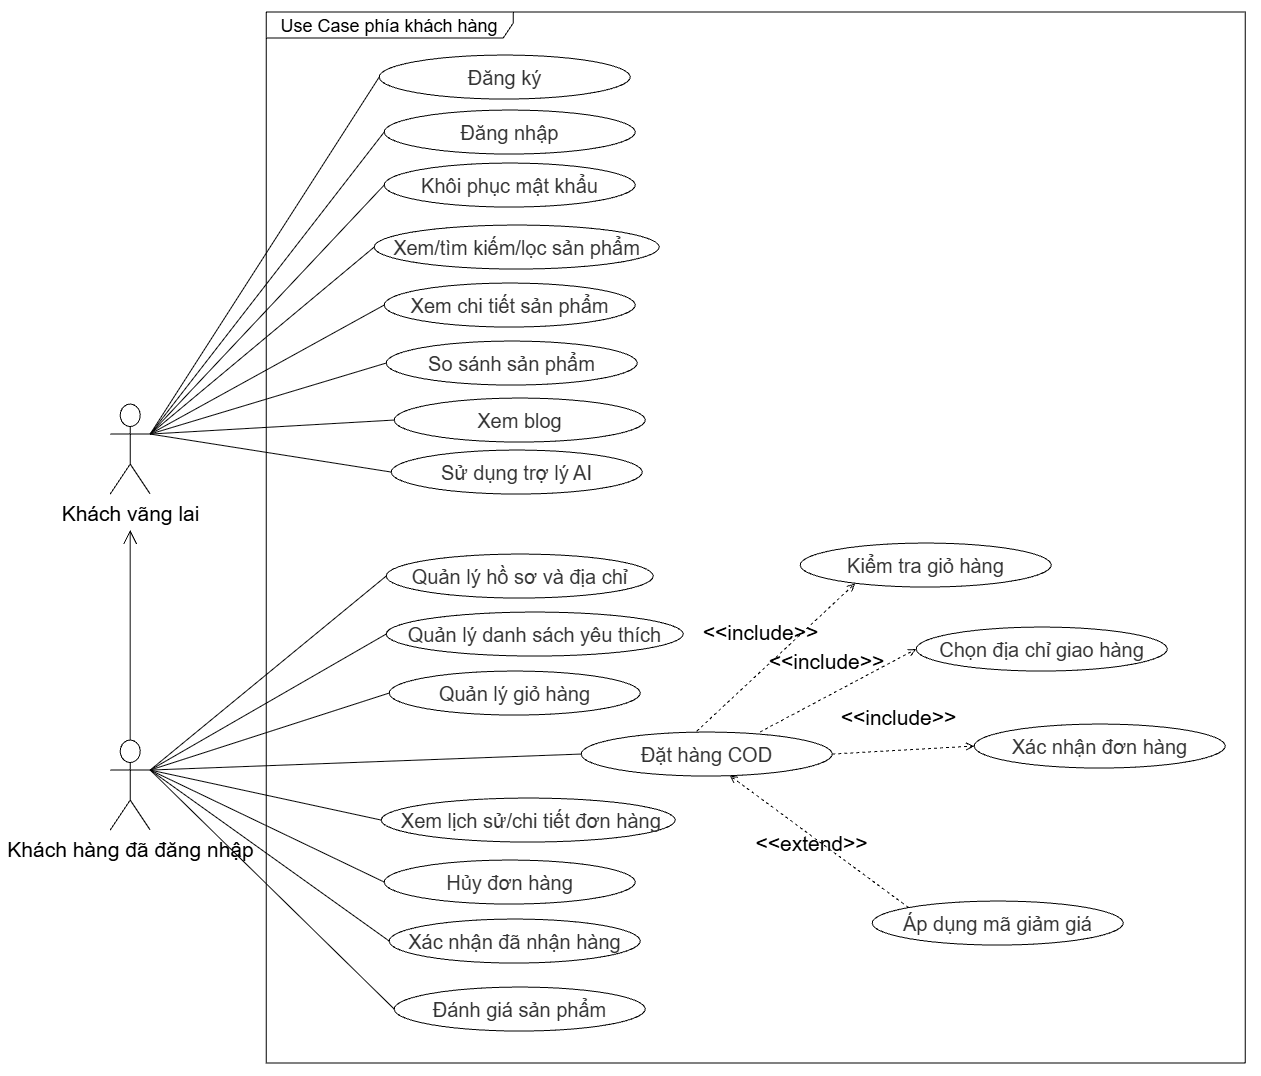
\includegraphics[width=0.74\textwidth,height=0.54\textheight,keepaspectratio]{Images/Usecase/da-Use Case phía khách hàng.drawio.png}
    \captionof{figure}{Sơ đồ Usecase phía khách hàng}
    \label{fig:usecase-customer}

\raggedright
Hình~\ref{fig:usecase-customer} phân biệt hai tác nhân là khách vãng lai và khách hàng đã
đăng nhập. Khách vãng lai có thể đăng ký, đăng nhập, khôi phục mật khẩu, tra cứu
sản phẩm, xem chi tiết, so sánh, đọc bài viết và sử dụng trợ lý AI. Khách hàng đã
đăng nhập kế thừa các khả năng này, đồng thời được quản lý hồ sơ, địa chỉ, danh
sách yêu thích, giỏ hàng và vòng đời đơn hàng.

Usecase đặt hàng COD bao gồm các bước bắt buộc là kiểm tra giỏ hàng, chọn địa chỉ
giao hàng và xác nhận đơn hàng; việc áp dụng mã giảm giá là nhánh mở rộng không bắt
buộc. Sau khi đặt hàng, người dùng có thể xem lịch sử, hủy đơn khi trạng thái cho
phép, xác nhận đã nhận hàng và đánh giá sản phẩm. Cách phân tách này làm rõ ranh
giới giữa chức năng công khai và nghiệp vụ cần xác thực.
\end{minipage}
\clearpage

\par\medskip\noindent
\begin{minipage}{\textwidth}
\textbf{Sơ đồ Usecase phía quản trị viên}

\centering
    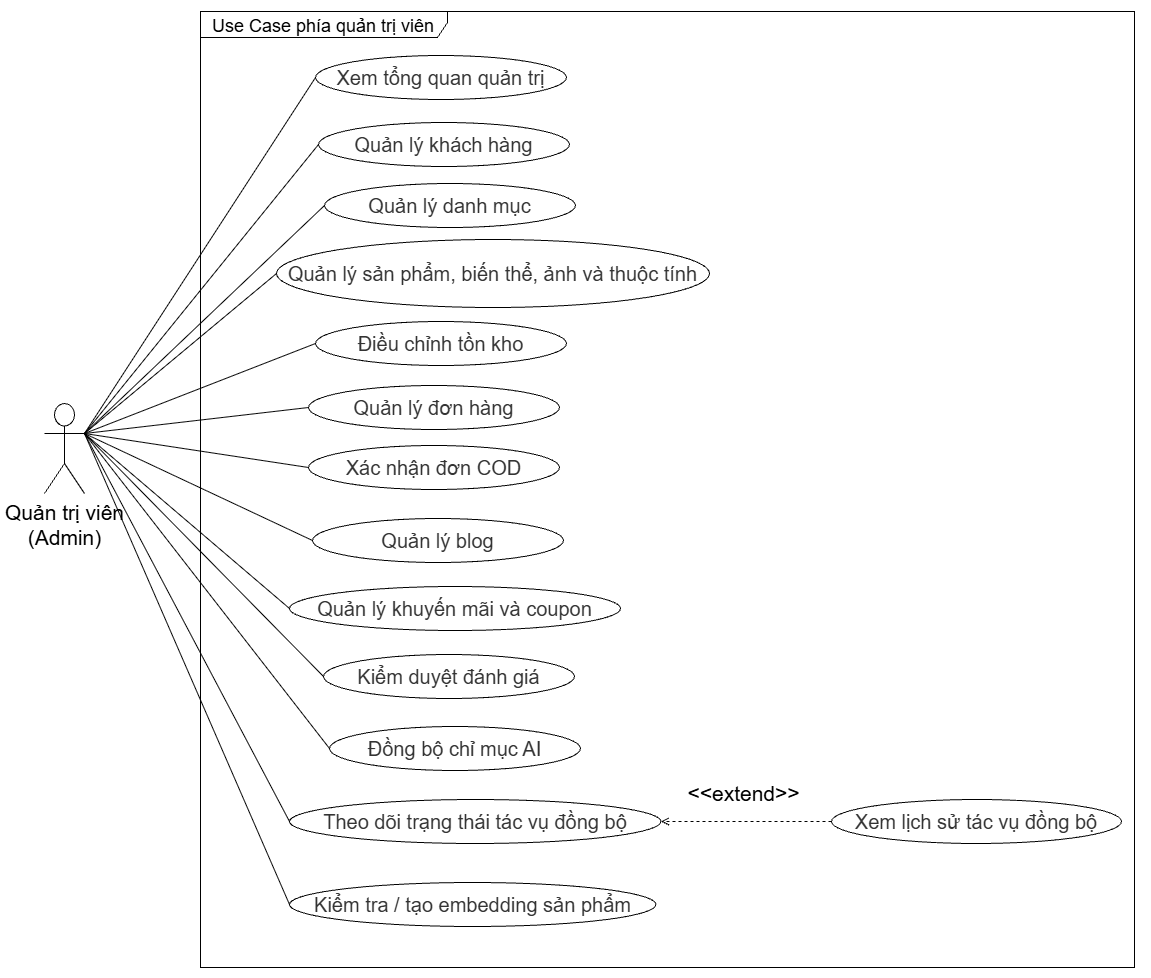
\includegraphics[width=0.74\textwidth,height=0.54\textheight,keepaspectratio]{Images/Usecase/da-Use Case phía quản trị viên.drawio.png}
    \captionof{figure}{Sơ đồ Usecase phía quản trị viên}
    \label{fig:usecase-admin}

\raggedright
Hình~\ref{fig:usecase-admin} tập trung các chức năng vận hành trong một vai trò đã
được xác thực và phân quyền. Nhóm quản trị nghiệp vụ bao gồm xem tổng quan, quản lý
khách hàng, danh mục, sản phẩm, biến thể, hình ảnh, thuộc tính, tồn kho, đơn hàng,
bài viết, khuyến mã, coupon và đánh giá. Trong quy trình đơn COD, quản trị viên tiếp
nhận, xác nhận và cập nhật đơn theo các chuyển trạng thái hợp lệ.

Nhóm vận hành AI cho phép khởi tạo đồng bộ chỉ mục, theo dõi trạng thái tác vụ và
kiểm tra hoặc tạo embedding sản phẩm. Xem lịch sử tác vụ là nhánh mở rộng của việc
theo dõi đồng bộ, giúp truy vết kết quả và lỗi mà không làm phức tạp luồng chính.
Mọi thao tác làm thay đổi dữ liệu hoặc trạng thái hệ thống đều phải qua kiểm tra quyền.
\end{minipage}
\clearpage

\par\medskip\noindent
\begin{minipage}{\textwidth}
\textbf{Sơ đồ Usecase của AI Service}

\centering
    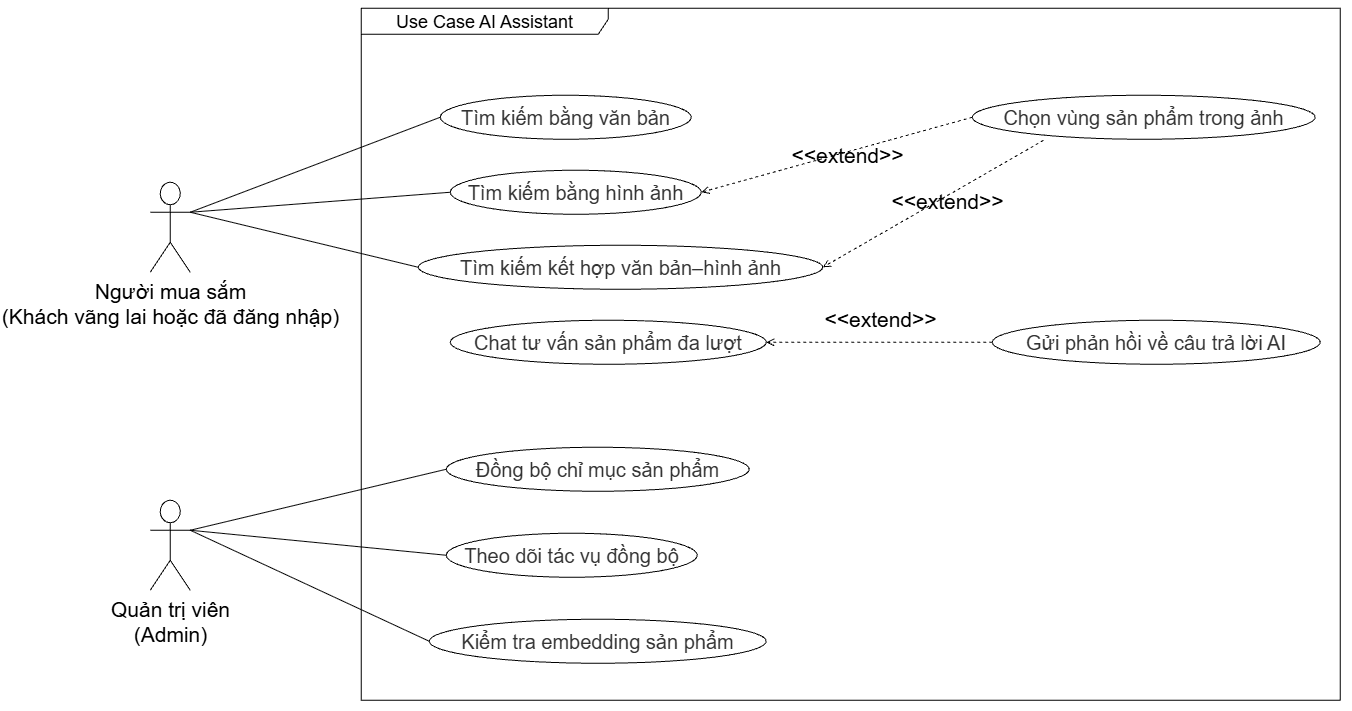
\includegraphics[width=0.84\textwidth,height=0.45\textheight,keepaspectratio]{Images/Usecase/da-Use Case AI Assistant.drawio.png}
    \captionof{figure}{Sơ đồ Usecase của AI Service}
    \label{fig:usecase-ai-assistant}

\raggedright
Hình~\ref{fig:usecase-ai-assistant} thể hiện hai nhóm tác nhân có mục tiêu khác nhau. Người mua sắm,
bao gồm cả khách vãng lai và người đã đăng nhập, sử dụng tìm kiếm bằng văn bản,
hình ảnh hoặc kết hợp hai phương thức; họ cũng có thể trao đổi nhiều lượt với trợ lý
để bổ sung và điều chỉnh nhu cầu. Chọn vùng sản phẩm trong ảnh là nhánh mở rộng
của tìm kiếm hình ảnh và tìm kiếm kết hợp, chỉ được thực hiện khi ảnh có nhiều đối
tượng hoặc người dùng muốn thu hẹp phạm vi truy vấn. Gửi phản hồi về câu trả lời AI là
nhánh tùy chọn sau khi hệ thống sinh phản hồi.

Quản trị viên không can thiệp trực tiếp vào kết quả truy vấn của từng người dùng mà chịu
trách nhiệm duy trì dữ liệu phục vụ AI. Các usecase quản trị gồm đồng bộ chỉ mục sản
phẩm, theo dõi tác vụ và kiểm tra embedding. Việc tách hai nhóm chức năng làm rõ ranh
giới giữa luồng phục vụ mua sắm và luồng quản trị chỉ mục nền.
\end{minipage}
\par\medskip

\FloatBarrier

\subsection{Sơ đồ hoạt động}

Ba sơ đồ hoạt động dưới đây đại diện cho luồng giao dịch, truy hồi đa phương
thức và hội thoại. Các sơ đồ xử lý đơn, đồng bộ chỉ mục và nhánh ngoại lệ chi
tiết được chuyển sang Phụ lục~\ref{appendix:analysis-model-detail}.

\par\medskip\noindent
\begin{minipage}{\textwidth}
Trong luồng đặt hàng, hệ thống kiểm tra giỏ hàng, tồn kho, địa chỉ và mã giảm
giá trước khi tạo đơn. Nếu một bước ghi dữ liệu bắt buộc thất bại, giao dịch
được rollback để không tạo ra đơn hàng không hoàn chỉnh.

\centering
    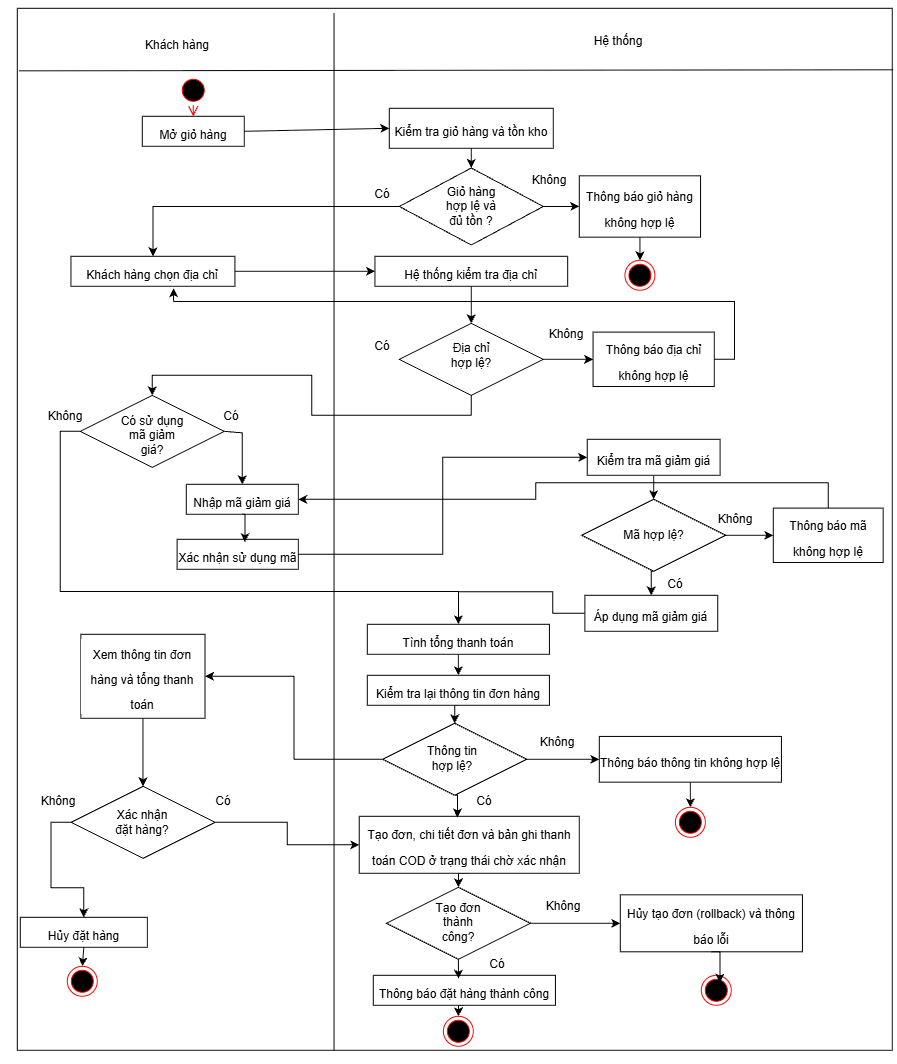
\includegraphics[width=1\textwidth,height=1\textheight,keepaspectratio]{Images/Activity/da-Đặt hàng COD.drawio.png}
    \captionof{figure}{Sơ đồ hoạt động đặt hàng COD}
    \label{fig:activity-cod-checkout}
\end{minipage}
\par\medskip

\par\medskip\noindent
\begin{minipage}{\textwidth}
AI Service định tuyến theo loại đầu vào và truy hồi trên collection tương ứng.
Với đầu vào ảnh--văn bản, hệ thống lọc ứng viên ảnh bằng ràng buộc trích từ văn
bản, chỉ dùng nhánh văn bản để phục hồi khi chưa đủ ứng viên, rồi xếp hạng theo
độ tương tự ảnh. Kết quả được đối chiếu với dữ liệu hiện hành trong MySQL trước
khi hiển thị cho người dùng.

\centering
    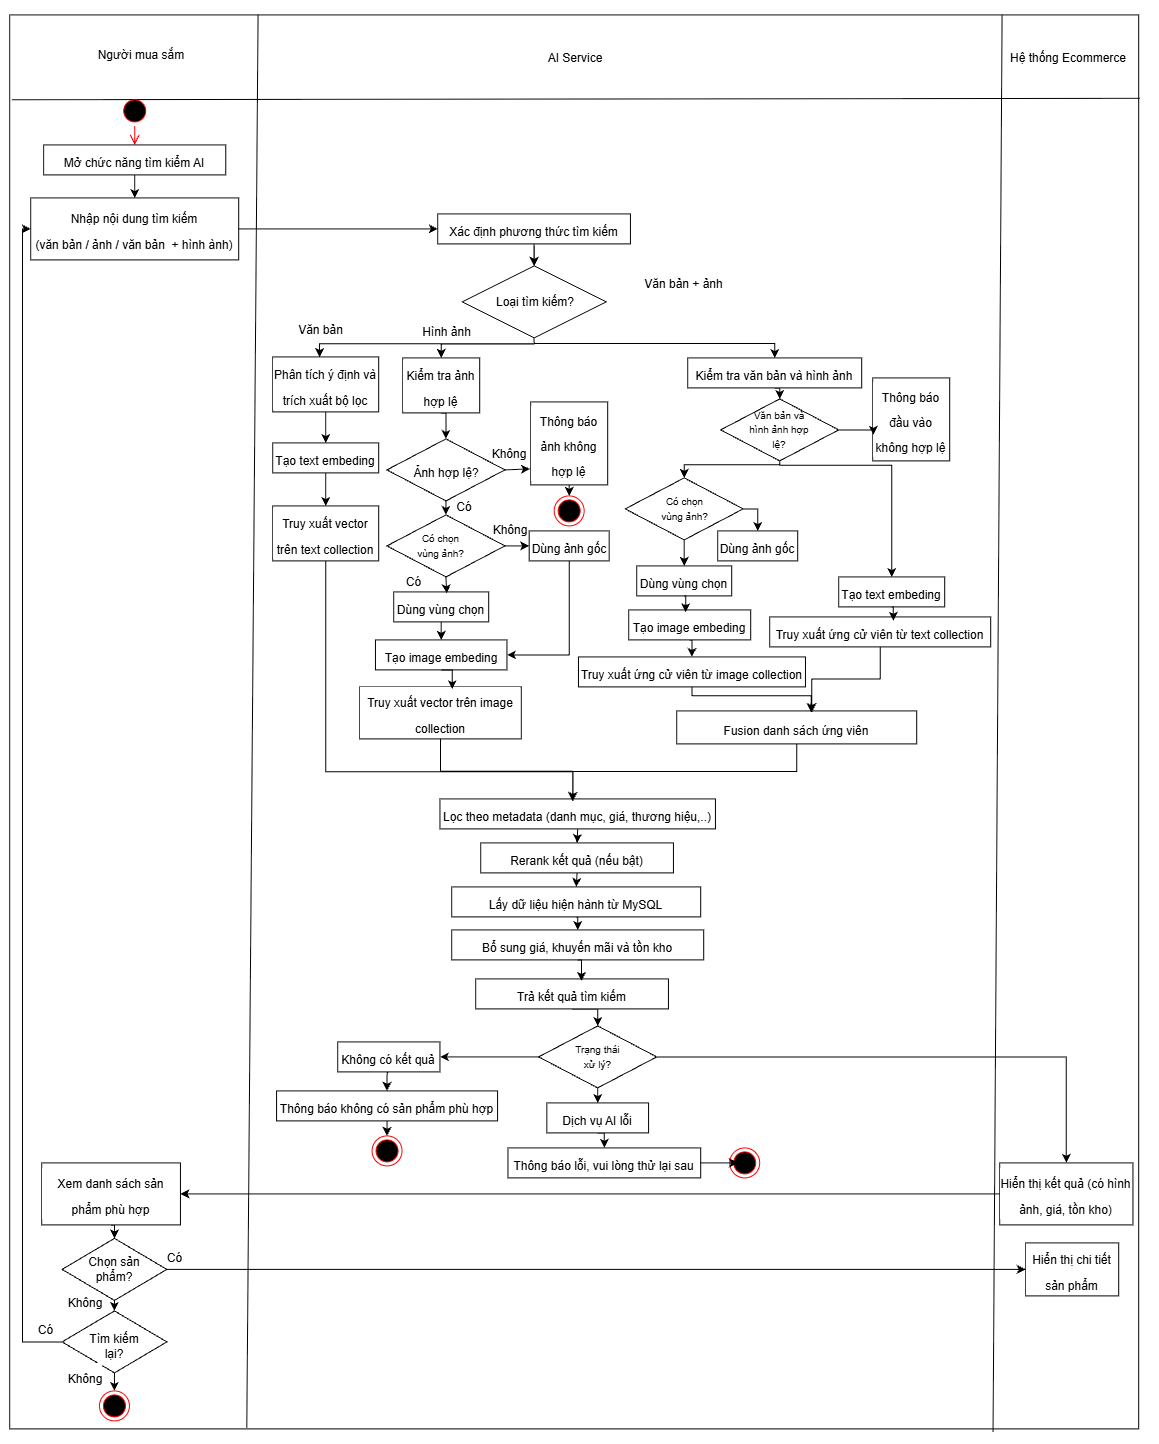
\includegraphics[width=1\textwidth,height=1\textheight,keepaspectratio]{Images/Activity/da-Tìm kiếm sản phẩm đa phương thức.drawio.png}
    \captionof{figure}{Sơ đồ hoạt động tìm kiếm sản phẩm đa phương thức}
    \label{fig:activity-multimodal-search}
\end{minipage}
\par\medskip

\par\medskip\noindent
\begin{minipage}{\textwidth}
Với hội thoại, hệ thống khôi phục bộ nhớ phiên, nhận diện ý định và truy hồi dữ
liệu sản phẩm khi cần. Phản hồi được tạo từ ngữ cảnh đã kiểm soát; trạng thái
cần thiết được lưu để phục vụ lượt trao đổi tiếp theo.

\centering
    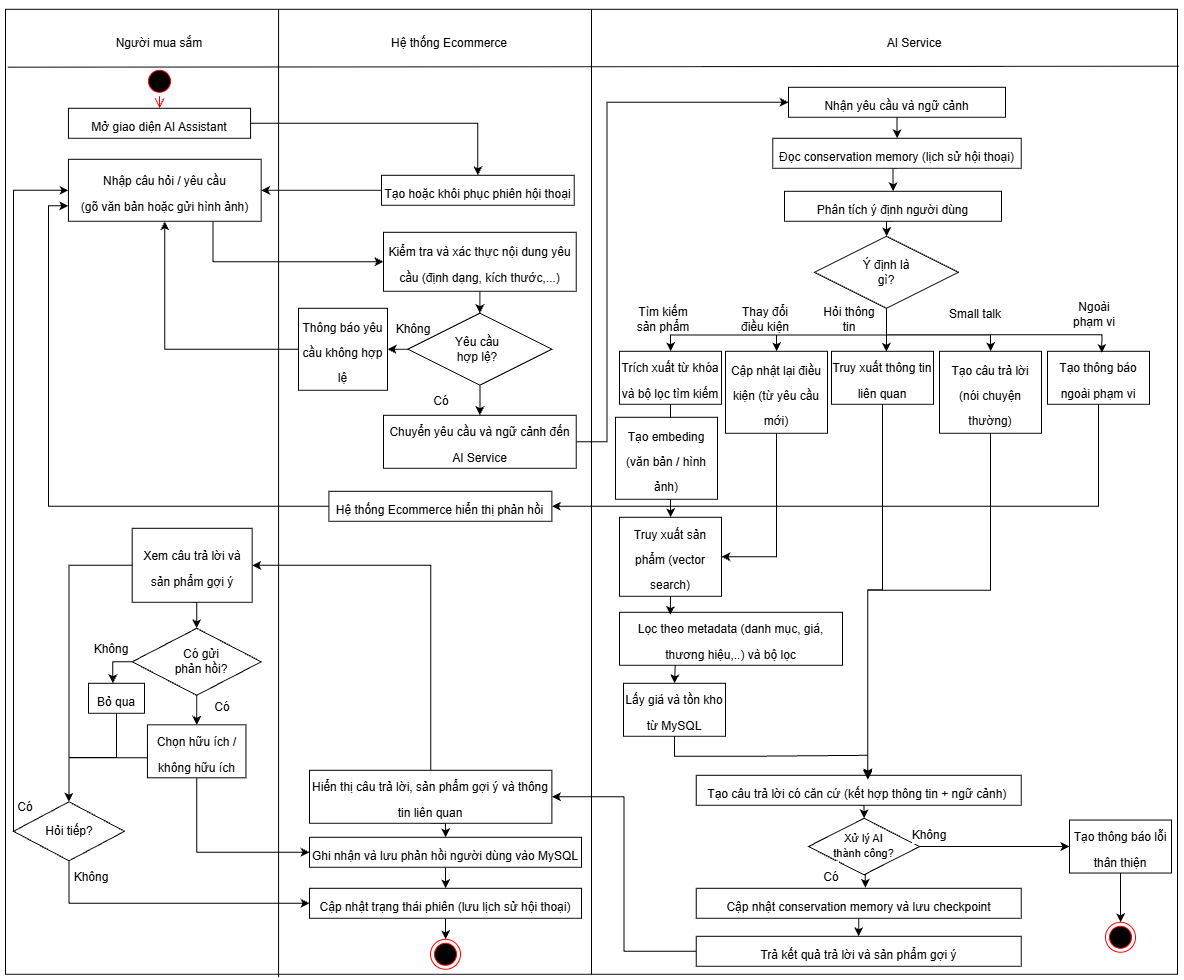
\includegraphics[width=1\textwidth,height=1\textheight,keepaspectratio]{Images/Activity/da-Chat tư vấn sản phẩm đa lượt.drawio.png}
    \captionof{figure}{Sơ đồ hoạt động tư vấn sản phẩm đa lượt}
    \label{fig:activity-multiturn-chat}
\end{minipage}
\par\medskip

\FloatBarrier

\subsection*{Kết chương}

Chương này đã xác định các bên liên quan, quy trình nghiệp vụ, yêu cầu chức
năng, yêu cầu dữ liệu và các thuộc tính phi chức năng của hệ thống. Các sơ đồ
Usecase và hoạt động làm rõ phạm vi chức năng cùng những luồng xử lý cốt lõi,
tạo cơ sở cho các chương thiết kế, hiện thực và kiểm thử.
